\documentclass[10.5pt]{jsarticle}
\usepackage{otf} %Windows上ではコメントアウト
\usepackage{amsmath, amssymb}
\usepackage[dvipdfmx]{graphics,xcolor}
\usepackage{tikz}
\usepackage[framemethod=tikz]{mdframed}
\usepackage{type1cm}
\usepackage{graphicx}
\usepackage{float}
\usepackage{here}
\usepackage{fancyhdr}
\usepackage{lscape} %ページ全体を用いた横向き画像使用時に使用

%マージン設定
%横
\setlength{\textwidth}{165truemm}
\setlength{\hoffset}{-1truein}
\setlength{\oddsidemargin}{25truemm}
%縦
\setlength{\textheight}{257truemm}
\setlength{\voffset}{-1truein}
\setlength{\topmargin}{10truemm}
\setlength{\headheight}{5truemm}
\setlength{\headsep}{5truemm}

%ページ番号設定
\pagestyle{fancy}
\fancyhead[RE]{}
\fancyhead[RO]{\thepage}
\fancyhead[LE]{\thepage}
\fancyhead[LO]{}
\cfoot{}
\renewcommand{\headrulewidth}{0pt}

%図表番号設定
%「図4.4.1」みたいにしたかったらsectionをsubsectionに変える
\makeatletter
\renewcommand{\figurename}{図}
\renewcommand{\thefigure}{\thesection.\arabic{figure}}
\@addtoreset{figure}{section}
\makeatother
\makeatletter
\renewcommand{\tablename}{表}
\renewcommand{\thetable}{\thesection.\arabic{table}}
\@addtoreset{table}{section}
\makeatother

%箇条書き表示設定
\renewcommand{\labelenumi}{(\arabic{enumi})}%第1階層
\renewcommand{\labelenumii}{(\roman{enumii})}%第2階層

%タイトル設定
\title{\LaTeXe 用テンプレート(片面印刷)}
\date{日付}
\author{作者}

%「jlisting.sty」が必要
\usepackage{listings,jlisting}
\def\lstlistingname{リスト}	%キャプションの設定
\lstset{%
language={Java},
basicstyle={\small},%
identifierstyle={\small},%
commentstyle={\small\itshape},%
keywordstyle={\small\bfseries},%
ndkeywordstyle={\small},%
stringstyle={\small\ttfamily},
frame={tb},
breaklines=true,
columns=[l]{fullflexible},%
numbers=left,%
xrightmargin=0zw,%
xleftmargin=3zw,%
numberstyle={\scriptsize},%
stepnumber=1,
numbersep=1zw,%
lineskip=-0.5ex%
}

\begin{document}

%タイトルの出力
\maketitle
\thispagestyle{fancy}

\section{実験日の天候,気温,湿度}
\begin{itemize}
	\item{2015/9/23(金)}
		\begin{itemize}
			\item[\textbf{天候:}]{雨}
			\item[\textbf{気温:}]{25$^\circ$C}
			\item[\textbf{湿度:}]{75\%}
		\end{itemize}
\end{itemize}

\section{目的}
本実験では・・・

\section{使用機材}
\begin{table}[H]
	\centering
	\caption{使用機材表} \label{Equipments}
	\begin{tabular}{|l|l|l|l|} 
		\hline
		\multicolumn{1}{|c|}{\textbf{名称}}&\multicolumn{1}{c|}{\textbf{メーカー}}&\multicolumn{1}{c|}{\textbf{型番}}&\multicolumn{1}{c|}{\textbf{数量}}\\\hline\hline
		AD/DA変換実習装置&IWATSU&ITF-203&1\\\hline
		直流電源装置&LEADER&818-3&1\\\hline
		直流電圧計&YOKOGAWA&2003&1\\\hline
	\end{tabular}
\end{table}

\newpage

\section{実験内容}
\subsection{実験1}
\subsubsection{実験手順}
\begin{enumerate}
\item{手順1}
	\begin{enumerate}
		\item{小手順1}
		\item{小手順2}
	\end{enumerate}
\item{手順2}
\end{enumerate}

\subsubsection{結果報告}
\begin{figure}[h]
	\centering
	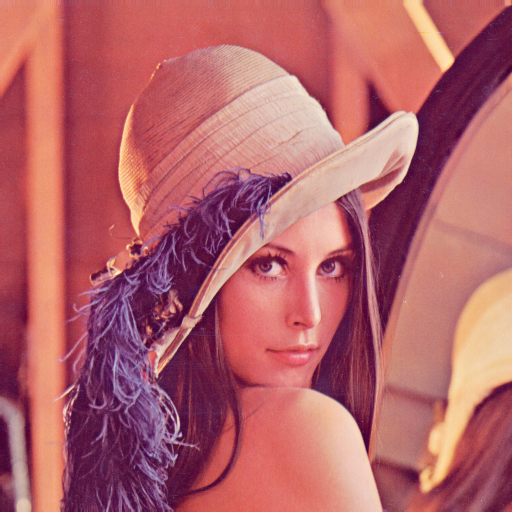
\includegraphics[width=0.4\hsize]{files/Lenna.png}
	\caption{キャプション}\label{ラベル}
\end{figure}
\begin{figure}[h]
	\begin{minipage}{0.5\hsize}
		\centering
		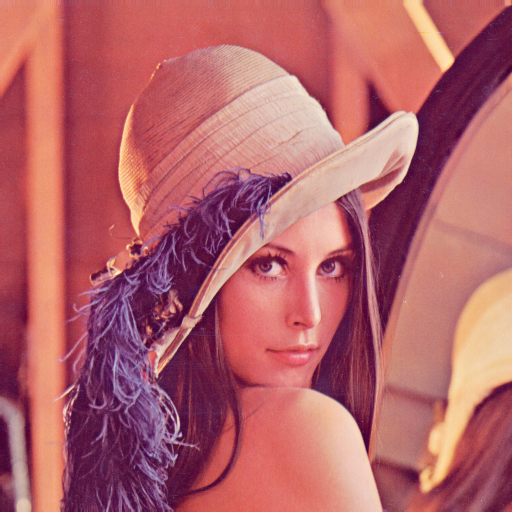
\includegraphics[width=0.8\hsize]{files/Lenna.png}\\
		(a)左
	\end{minipage}
	\begin{minipage}{0.5\hsize}
		\centering
		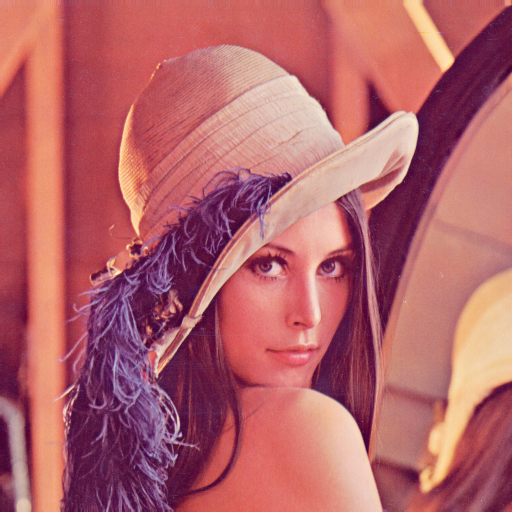
\includegraphics[width=0.8\hsize]{files/Lenna.png}\\
		(b)右
	\end{minipage}
	\caption{並べて表示}
\end{figure}

\section{検討}
\subsection{検討事項1}
\begin{align}
x+1&=3 \notag \\
x&=2
\end{align}

\section{考察}

%参考文献の明示
\begin{flushright}
	\cite{4GT}
	\cite{TCP/IP}
\end{flushright}

\begin{thebibliography}{999}%文献数の桁数に応じて9の数を変える(変えなくてもよい)
	\bibitem{4GT} 「4-Gigabyte Tuning: BCDEdit and Boot.ini (Windows)」 - https://msdn.microsoft.com/ja-jp/library/windows/desktop/bb613473(v=vs.85).aspx, 2015年6月23日にアクセス
	\bibitem{TCP/IP} 谷口功 『図解入門 最新TCP/IPの基本と仕組み』 (秀和システム, 2011) pp.62-111, pp.202-228
\end{thebibliography}

\appendix
\section{ソースコード}
%直接書く場合
\begin{lstlisting}[caption=キャプション,label=ラベル]
class HelloWorld{
	public static void main(String[] args){  
		System.out.println("Hello, World!");
	}
}
\end{lstlisting}
%ファイルから直接指定する場合
\lstinputlisting[caption=HelloWorld.java,label=ラベル]{files/HelloWorld.java}
\end{document}
